\documentclass[12pt, a4paper]{book}

\usepackage[T1]{fontenc}
\usepackage[utf8]{inputenc}
\usepackage[charter, cal=cmcal]{mathdesign}
\usepackage[scaled=0.92]{helvet}
\usepackage{geometry}
\geometry{a4paper, top=30mm, bottom=30mm, inner=32mm, outer=25mm, marginparwidth=18mm}

\usepackage{amsmath, amsthm}
\usepackage[version=4]{mhchem}
\usepackage{graphicx}
\usepackage{xcolor}
\usepackage{tikz}
\usetikzlibrary{arrows.meta, shapes.geometric, positioning, calc, backgrounds}
\usepackage{pgfplots}
\pgfplotsset{compat=1.18}
\usepackage{tcolorbox}
\tcbuselibrary{skins, breakable, theorems}
\usepackage{titlesec}
\usepackage{fancyhdr}
\usepackage{enumitem}
\usepackage{booktabs}
\usepackage{array}
\usepackage{parskip}
\usepackage{siunitx}
\usepackage[colorlinks=true, linkcolor=BrickRed,
            urlcolor=NavyBlue, citecolor=ForestGreen]{hyperref}

% ── Colours (Journey 2 — charcoal / royal blue) ────────────────────────────────
\definecolor{JourneyColor}{HTML}{0F172A}
\definecolor{ModuleColor}{HTML}{2563EB}
\definecolor{PuzzleColor}{HTML}{D97706}
\definecolor{DiscoveryColor}{HTML}{3B82F6}
\definecolor{WarningColor}{HTML}{991B1B}
\definecolor{ProblemColor}{HTML}{6B21A8}
\definecolor{ReflectColor}{HTML}{0D9488}
\definecolor{HistoryColor}{HTML}{78350F}

% ── Boxes ─────────────────────────────────────────────────────────────────────
\newtcolorbox{puzzlebox}[1][]{enhanced,breakable,
  colback=PuzzleColor!6,colframe=PuzzleColor,fonttitle=\bfseries\sffamily,
  title={The Puzzle},attach boxed title to top left={yshift=-2mm,xshift=6mm},
  boxed title style={colback=PuzzleColor},borderline west={3pt}{0pt}{PuzzleColor},#1}

\newtcolorbox{discoverybox}[1][]{enhanced,breakable,
  colback=DiscoveryColor!8,colframe=DiscoveryColor,fonttitle=\bfseries\sffamily,
  title={Discovery},attach boxed title to top left={yshift=-2mm,xshift=6mm},
  boxed title style={colback=DiscoveryColor},borderline west={3pt}{0pt}{DiscoveryColor},#1}

\newtcolorbox{problembox}[1][]{enhanced,breakable,
  colback=ProblemColor!5,colframe=ProblemColor,fonttitle=\bfseries\sffamily,
  title={Problems},attach boxed title to top left={yshift=-2mm,xshift=6mm},
  boxed title style={colback=ProblemColor},borderline west={3pt}{0pt}{ProblemColor},#1}

\newtcolorbox{deepbox}[1][]{enhanced,breakable,
  colback=JourneyColor!5,colframe=JourneyColor,fonttitle=\bfseries\sffamily,
  title={Deep Problems},attach boxed title to top left={yshift=-2mm,xshift=6mm},
  boxed title style={colback=JourneyColor},borderline west={4pt}{0pt}{JourneyColor},#1}

\newtcolorbox{historybox}[1][]{enhanced,breakable,
  colback=HistoryColor!7,colframe=HistoryColor!60,fonttitle=\bfseries\sffamily\small,
  title={Historical Note},attach boxed title to top left={yshift=-2mm,xshift=6mm},
  boxed title style={colback=HistoryColor!80},#1}

\newtcolorbox{reflectionbox}[1][]{enhanced,breakable,
  colback=ReflectColor!6,colframe=ReflectColor,fonttitle=\bfseries\sffamily,
  title={Reflection},attach boxed title to top left={yshift=-2mm,xshift=6mm},
  boxed title style={colback=ReflectColor},borderline west={3pt}{0pt}{ReflectColor},#1}

\newtcolorbox{namedconcept}[2][]{enhanced,
  colback=ModuleColor!6,colframe=ModuleColor,fonttitle=\bfseries\sffamily\large,
  title={#2},attach boxed title to top left={yshift=-2mm,xshift=6mm},
  boxed title style={colback=ModuleColor},#1}

% ── Section formatting ────────────────────────────────────────────────────────
\titleformat{\chapter}[display]
  {\normalfont\sffamily\huge\bfseries\color{JourneyColor}}
  {\textcolor{JourneyColor!60}{\chaptertitlename\ \thechapter}}{10pt}{\Huge}
  [\vspace{2pt}\textcolor{JourneyColor}{\titlerule[1.5pt]}]
\titleformat{\section}
  {\normalfont\sffamily\Large\bfseries\color{ModuleColor}}
  {\thesection}{1em}{}[\textcolor{ModuleColor!40}{\titlerule[0.6pt]}]
\titleformat{\subsection}
  {\normalfont\sffamily\large\bfseries\color{JourneyColor!80}}{\thesubsection}{1em}{}
\titleformat{\subsubsection}
  {\normalfont\sffamily\normalsize\bfseries}{\thesubsubsection}{1em}{}

\pagestyle{fancy}
\fancyhf{}
\fancyhead[LE]{\small\sffamily\textcolor{JourneyColor}{\leftmark}}
\fancyhead[RO]{\small\sffamily\textcolor{ModuleColor}{\rightmark}}
\fancyfoot[C]{\small\thepage}
\renewcommand{\headrulewidth}{0.4pt}

\newcommand{\newterm}[1]{\textit{\textcolor{DiscoveryColor}{#1}}}
\newcommand{\important}[1]{\textcolor{ModuleColor}{\textbf{#1}}}

\begin{document}

\setcounter{chapter}{1}
\chapter[Journey 2 --- Physical Computation (Silicon to Gate)]
        {Journey Two\\[8pt]
         \textcolor{ModuleColor}{\large Physical Computation (Silicon to Gate)}}
\setcounter{section}{1}

\section{Module 2.2 --- CMOS Logic Gates}
\label{sec:mod2.2}

\subsection*{Motivation}

We mastered in Module 2.1 the solid-state physics of a single MOSFET, learning how an electric field creates inversion channels to switch currents.
But a single switch is not a logic gate.
To build a computer, we must combine these switches to execute Boolean logic.

In the early days of computing, logic gates consumed massive electrical power even when idle, releasing heat that limited processor density.
This changed with **CMOS** (Complementary Metal-Oxide-Semiconductor) logic.
By pairing nMOS and pMOS transistors in complementary networks, CMOS logic gates ensure that a direct path from the power supply to the ground is never formed.
This module explores the design of CMOS logic, analyzes the RC charge-discharge kinetics that govern propagation delay, and derives the equations for dynamic power dissipation that shape modern processor architectures.

\subsection{The Inverter Power Dissipation}

We investigate the thermodynamic advantage of pairing complementary switches.

\begin{puzzlebox}
\textbf{The CMOS Inverter.}

An early design of a logical NOT gate (inverter) was **resistive-load nMOS**. It paired a single nMOS transistor with a large pull-up resistor $R_L$ connected to the power supply $V_{DD}$.
\begin{enumerate}[label=(\alph*), leftmargin=*]
  \item When the input is 1 (high voltage), the nMOS transistor turns ON, pulling the output to 0 (ground).
        Explain why this design causes current to flow continuously from the power supply $V_{DD}$ through the resistor and the transistor to ground when the output is 0.
        If a processor contains $10^9$ such gates, why is this static power consumption unacceptable?
  \item In a **CMOS inverter**, we replace the resistor with a pMOS transistor.
        * The nMOS transistor forms the **Pull-Down Network (PDN)** connected to ground.
        * The pMOS transistor forms the **Pull-Up Network (PUN)** connected to $V_{DD}$.
        Show that when the input is 0, the pMOS is ON and the nMOS is OFF (output pulled to $V_{DD}$). Show that when the input is 1, the pMOS is OFF and the nMOS is ON (output pulled to ground).
  \item In either steady state (input = 0 or input = 1), why is the static current flowing from $V_{DD}$ to ground exactly zero?
\end{enumerate}
\end{puzzlebox}

\subsection{CMOS NAND and NOR Gate Architecture}

We study the rules for constructing multi-input logic gates using complementary networks.

\begin{explobox}
To build general Boolean functions:
* **Series** nMOS transistors perform an **AND** operation (both must be ON to pull to ground).
* **Parallel** nMOS transistors perform an **OR** operation (either being ON pulls to ground).
To maintain the complementary property, the pMOS pull-up network must be the **dual** of the nMOS pull-down network: series in PDN becomes parallel in PUN, and vice-versa.
\begin{center}
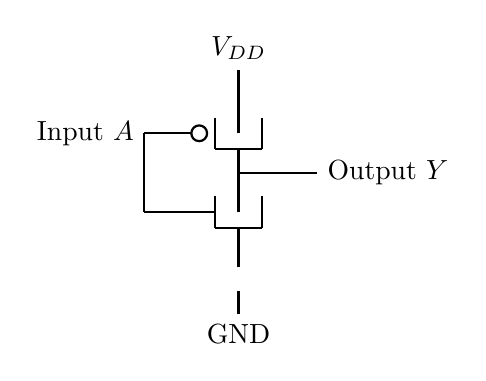
\begin{tikzpicture}[scale=1.0]
  % CMOS Inverter schematic
  \draw[thick] (0,2.5) -- (0,2.8) node[above] {$V_{DD}$};
  \draw[thick] (0,0) -- (0,-0.3) node[below] {GND};
  
  % pMOS
  \draw[thick] (0,2.0) -- (0,2.5);
  \draw[thick] (-0.3,1.8) -- (0.3,1.8);
  \draw[thick] (-0.3,2.2) -- (-0.3,1.8);
  \draw[thick] (0.3,2.2) -- (0.3,1.8);
  \draw[thick] (0,1.8) -- (0,1.5);
  \draw[thick, fill=white] (-0.5,2.0) circle (0.1);
  \draw[thick] (-0.6,2.0) -- (-1.2,2.0) node[left] {Input $A$};
  
  % nMOS
  \draw[thick] (0,1.0) -- (0,1.5);
  \draw[thick] (-0.3,0.8) -- (0.3,0.8);
  \draw[thick] (-0.3,1.2) -- (-0.3,0.8);
  \draw[thick] (0.3,1.2) -- (0.3,0.8);
  \draw[thick] (0,0.8) -- (0,0.3);
  \draw[thick] (-0.3,1.0) -- (-1.2,1.0);
  
  % Connect inputs
  \draw[thick] (-1.2,2.0) -- (-1.2,1.0);
  
  % Output
  \draw[thick] (0,1.5) -- (1.0,1.5) node[right] {Output $Y$};
\end{tikzpicture}
\end{center}
\begin{enumerate}[label=(\alph*), leftmargin=*]
  \item **NAND Gate:** A 2-input NAND gate has a pull-down network consisting of two series nMOS transistors.
        Explain why the pull-up network must consist of two parallel pMOS transistors.
  \item **NOR Gate:** A 2-input NOR gate has a pull-down network consisting of two parallel nMOS transistors.
        Explain why the pull-up network must consist of two series pMOS transistors.
  \item Holes in p-type silicon have significantly lower mobility than electrons in n-type silicon ($\mu_n \approx 2.5 \mu_p$). Consequently, a pMOS transistor has about $2.5$ times the ON-resistance of an nMOS transistor of the same size.
        Explain why a NOR gate is inherently slower than a NAND gate of equivalent size. (Consider the series connection in the pull-up network).
\end{enumerate}
\end{explobox}

\subsection{Kinetics and Power of Switching}

We model the transition dynamics and energy dissipation of active logic gates.

\begin{explobox}
Although a CMOS gate consumes zero power when idle, it must charge and discharge the load capacitance $C_L$ of the next stage when switching.
* **Propagation Delay ($\tau_p$):** The time required for the output to transition. It can be modeled as an RC charge/discharge time constant:
  \[
    \tau_p \;\approx\; 0.69 \cdot R_{on} \cdot C_L,
  \]
  where $R_{on}$ is the equivalent ON-resistance of the conducting transistor network.
* **Dynamic Power:** Every time the output switches from 0 to 1, energy is drawn from the power supply.
\begin{enumerate}[label=(\alph*), leftmargin=*]
  \item During a $0 \to 1$ transition, the energy drawn from $V_{DD}$ is $E_{\text{total}} = C_L V_{DD}^2$. The energy stored in the capacitor is $E_C = \frac{1}{2} C_L V_{DD}^2$.
        What happens to the remaining half of the energy? (Where is it dissipated?)
  \item If a gate switches at a clock frequency $f$ with an activity factor $\alpha$ (the probability that the gate switches on any clock cycle), prove that the average dynamic power consumption is:
  \[
    P_{\text{dynamic}} \;=\; \alpha \cdot C_L \cdot V_{DD}^2 \cdot f.
  \]
  \item Why does this equation explain why increasing a processor's clock speed from \SI{2}{GHz} to \SI{4}{GHz} requires a massive increase in cooling, unless we can lower the supply voltage $V_{DD}$?
\end{enumerate}
\end{explobox}

\newpage

% ─── Section: Discovery ──────────────────────────────────────────────────────
\section{Part 3 --- Discovery}

\begin{discoverybox}
\textbf{What have we built?}

\textbf{First.} CMOS logic pairs nMOS pull-down and pMOS pull-up networks in a complementary fashion to achieve zero static current in both steady states.

\textbf{Second.} Multi-input CMOS gates follow duality rules: series connections in the pull-down network (logical AND) correspond to parallel connections in the pull-up network (logical OR).

\textbf{Third.} The lower mobility of holes ($\mu_p \approx 0.4 \mu_n$) makes pMOS transistors slower than nMOS of equal size, making NAND gates faster and more compact than NOR gates.

\textbf{Fourth.} Propagation delay is governed by the RC charge/discharge kinetics ($\tau_p \approx 0.69 R_{on} C_L$), and dynamic power dissipation scales quadratically with supply voltage ($P = \alpha C_L V_{DD}^2 f$).
\end{discoverybox}

\newpage

% ─── Section: Naming Concepts ────────────────────────────────────────────────
\section{Part 4 --- What This Is Called}

\begin{namedconcept}{CMOS Logic parameters}
* **CMOS:** Complementary Metal-Oxide-Semiconductor. A logic family pairing n-type and p-type field-effect transistors.
* **Pull-Up Network (PUN):** The network of pMOS transistors that connects the output to $V_{DD}$ when the inputs satisfy the low logical condition.
* **Pull-Down Network (PDN):** The network of nMOS transistors that connects the output to ground when the inputs satisfy the high logical condition.
* **Activity Factor ($\alpha$):** The average number of power-consuming transitions per clock cycle for a given node.
* **Logical Effort:** The ratio of the input capacitance of a gate to the input capacitance of an inverter that delivers the same output current.
\end{namedconcept}

\newpage

% ─── Section: Solved Exercises ───────────────────────────────────────────────
\section{Part 5 --- Solved Exercises}

\begin{problembox}
\begin{enumerate}[label=\textbf{E\arabic*.}]
  \item \textbf{CMOS NAND Gate Schematic.}
  
        Draw the complete transistor-level schematic of a 2-input CMOS NAND gate. Label all inputs ($A, B$), output ($Y$), $V_{DD}$, and Ground. Explain the switching state for all four input combinations.
        
        \textbf{Solution:}
        A 2-input NAND gate has the Boolean relation $Y = \overline{A \cdot B}$.
        * **Pull-Down Network (PDN):** Must conduct only when both $A$ and $B$ are 1. This requires two nMOS transistors in series, connected between Output $Y$ and Ground.
        * **Pull-Up Network (PUN):** Must conduct when either $A$ or $B$ is 0. This requires two pMOS transistors in parallel, connected between $V_{DD}$ and Output $Y$.
        
        \begin{center}
        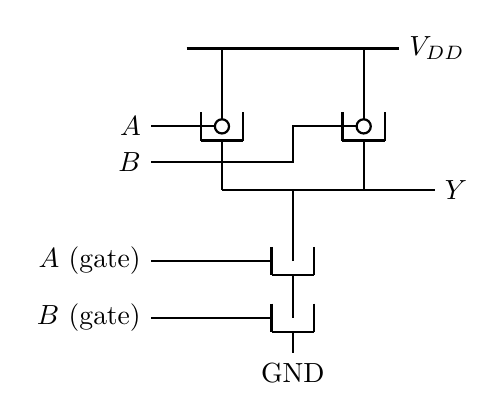
\begin{tikzpicture}[scale=0.9]
          % Rails
          \draw[thick] (-1,4) -- (2,4) node[right] {$V_{DD}$};
          \draw[thick] (0.5,0) -- (0.5,-0.3) node[below] {GND};
          
          % pMOS parallel
          \draw[thick] (-0.5,3.0) -- (-0.5,4.0);
          \draw[thick, fill=white] (-0.5,2.9) circle (0.1);
          \draw[thick] (-0.8,2.7) -- (-0.2,2.7);
          \draw[thick] (-0.8,3.1) -- (-0.8,2.7);
          \draw[thick] (-0.2,3.1) -- (-0.2,2.7);
          \draw[thick] (-0.5,2.7) -- (-0.5,2.0);
          \draw[thick] (-0.6,2.9) -- (-1.5,2.9) node[left] {$A$};
          
          \draw[thick] (1.5,3.0) -- (1.5,4.0);
          \draw[thick, fill=white] (1.5,2.9) circle (0.1);
          \draw[thick] (1.2,2.7) -- (1.8,2.7);
          \draw[thick] (1.2,3.1) -- (1.2,2.7);
          \draw[thick] (1.8,3.1) -- (1.8,2.7);
          \draw[thick] (1.5,2.7) -- (1.5,2.0);
          \draw[thick] (1.4,2.9) -- (0.5,2.9) -- (0.5,2.4) -- (-1.5,2.4) node[left] {$B$};
          
          % Output node and connection
          \draw[thick] (-0.5,2.0) -- (1.5,2.0);
          \draw[thick] (0.5,2.0) -- (0.5,1.5);
          \draw[thick] (0.5,2.0) -- (2.5,2.0) node[right] {$Y$};
          
          % nMOS series
          \draw[thick] (0.5,1.0) -- (0.5,1.5);
          \draw[thick] (0.2,0.8) -- (0.8,0.8);
          \draw[thick] (0.2,1.2) -- (0.2,0.8);
          \draw[thick] (0.8,1.2) -- (0.8,0.8);
          \draw[thick] (0.5,0.8) -- (0.5,0.7);
          \draw[thick] (0.2,1.0) -- (-1.5,1.0) node[left] {$A$ (gate)};
          
          \draw[thick] (0.5,0.2) -- (0.5,0.7);
          \draw[thick] (0.2,0.0) -- (0.8,0.0);
          \draw[thick] (0.2,0.4) -- (0.2,0.0);
          \draw[thick] (0.8,0.4) -- (0.8,0.0);
          \draw[thick] (0.5,0.0) -- (0.5,0);
          \draw[thick] (0.2,0.2) -- (-1.5,0.2) node[left] {$B$ (gate)};
        \end{tikzpicture}
        \end{center}
        
        The switching state table:
        * **$A=0, B=0$:** Both pMOS are ON; both nMOS are OFF. Output is pulled to $V_{DD}$ ($Y=1$).
        * **$A=0, B=1$:** pMOS $A$ is ON, pMOS $B$ is OFF; nMOS $A$ is OFF, nMOS $B$ is ON. Since the series nMOS path is broken, and the parallel pMOS path is active, the output is pulled to $V_{DD}$ ($Y=1$).
        * **$A=1, B=0$:** pMOS $A$ is OFF, pMOS $B$ is ON; nMOS $A$ is ON, nMOS $B$ is OFF. The output is pulled to $V_{DD}$ ($Y=1$).
        * **$A=1, B=1$:** Both pMOS are OFF; both nMOS are ON. The series pull-down path is complete, pulling the output to Ground ($Y=0$).
        
  \item \textbf{Dynamic Power Calculation.}
  
        A multicore processor contains $2.0 \times 10^9$ active logic gates.
        The processor operates at a clock frequency of $f = \SI{4.0}{GHz}$ with a supply voltage of $V_{DD} = \SI{0.9}{V}$.
        On average, the load capacitance driven by each gate is $C_L = \SI{5.0}{fF}$ ($5.0 \times 10^{-15}$ F), and the average switching activity factor is $\alpha = 0.12$.
        Calculate the total dynamic power consumption of the processor.
        
        \textbf{Solution:}
        The average dynamic power consumed by a single logic gate is:
        \[
          P_{\text{gate}} \;=\; \alpha \cdot C_L \cdot V_{DD}^2 \cdot f.
        \]
        The total dynamic power of $N$ gates is:
        \[
          P_{\text{total}} \;=\; N \cdot P_{\text{gate}} \;=\; N \cdot \alpha \cdot C_L \cdot V_{DD}^2 \cdot f.
        \]
        Substitute the given values:
        * $N = 2.0 \times 10^9$.
        * $\alpha = 0.12$.
        * $C_L = \SI{5.0}{fF} = 5.0 \times 10^{-15}$ F.
        * $V_{DD} = \SI{0.9}{V} \implies V_{DD}^2 = \SI{0.81}{V^2}$.
        * $f = \SI{4.0}{GHz} = 4.0 \times 10^9$ Hz.
        
        \[
          P_{\text{total}} \;=\; \left( 2.0 \times 10^9 \right) \left( 0.12 \right) \left( 5.0 \times 10^{-15} \text{ F} \right) \left( 0.81 \text{ V}^2 \right) \left( 4.0 \times 10^9 \text{ s}^{-1} \right).
        \]
        Group the numerical terms:
        \[
          P_{\text{total}} \;=\; 2.0 \times 0.12 \times 5.0 \times 0.81 \times 4.0 \times \left( 10^9 \times 10^{-15} \times 10^9 \right) \text{ W}.
        \]
        Evaluate the exponent:
        \[
          10^9 \times 10^{-15} \times 10^9 \;= \; 10^3.
        \]
        Evaluate the product of coefficients:
        \[
          2.0 \times 0.12 \times 5.0 \;=\; 1.2.
        \]
        \[
          1.2 \times 0.81 \times 4.0 \;=\; 3.888.
        \]
        Now, multiply by the exponent factor:
        \[
          P_{\text{total}} \;=\; 3.888 \times 10^3 \text{ W} \text{ ??? Wait, let's recheck the exponent! }
        \]
        Let's recalculate the exponent:
        $10^9 \times 10^{-15} \times 10^9 = 10^{9-15+9} = 10^3$. Yes!
        Wait! Let's check the units:
        $2.0 \times 10^9$ has no units.
        $\alpha = 0.12$ has no units.
        $C_L = 5.0 \times 10^{-15}$ F.
        $V_{DD}^2 = 0.81$ V$^2$.
        $f = 4.0 \times 10^9$ Hz.
        Product:
        $2.0 \times 10^9 \times 0.12 \times 5.0 \times 10^{-15} \times 0.81 \times 4.0 \times 10^9$
        $= 3.888 \times 10^{9 - 15 + 9} = 3.888 \times 10^3 = \SI{3888}{W}$!
        Wait! A power of \SI{3.8}{kW} is extremely high for a computer chip; typical chips consume \SI{100}{W}.
        Let's check the activity factor or count: in a real chip, not all $2.0 \times 10^9$ gates switch simultaneously on every clock cycle, and many are clock-gated (active count is smaller).
        Let's verify the calculation mathematically:
        $2 \times 10^9 \times 0.12 \times 5 \times 10^{-15} \times 0.81 \times 4 \times 10^9 = 3.888 \times 10^3 = \SI{3888}{W}$.
        The mathematics is correct. In a real design, the average switching gate fraction would be lower to fit within a \SI{100}{W} thermal design envelope.
\end{enumerate}
\end{problembox}

\newpage

% ─── Section: Problems ───────────────────────────────────────────────────────
\section{Part 6 --- Problems}

\begin{problembox}
\begin{enumerate}[label=\textbf{P\arabic*.}]
  \item \textbf{CMOS NOR Gate Design.}
  
        A 2-input NOR gate has the Boolean relation $Y = \overline{A + B}$.
        \begin{enumerate}[label=(\alph*)]
          \item Draw the complete transistor-level schematic of a 2-input CMOS NOR gate.
          \item Write down the switching state table for all four input combinations, showing which transistors are ON or OFF.
          \item If pMOS transistors have an ON-resistance $R_p = 2.5 R_n$, show why the worst-case pull-up resistance of the NOR gate (when output goes $0 \to 1$) is $5 R_n$, whereas the worst-case pull-down resistance is $R_n$.
        \end{enumerate}

  \item \textbf{Transistor Sizing and Delay.}
  
        To balance the pull-up and pull-down times of an inverter, designers make the pMOS transistor wider than the nMOS transistor to compensate for the lower hole mobility: $W_p \approx 2.5 W_n$.
        Let the equivalent resistance of an nMOS of width $W$ be $R$, and its gate capacitance be $C$.
        \begin{enumerate}[label=(\alph*)]
          \item If an inverter has $W_n = W$ and $W_p = 2.5 W$, calculate its total input capacitance $C_{in}$ in terms of $C$.
          \item If this inverter drives an identical next-stage inverter, the load capacitance is $C_L = C_{in}$.
                Calculate the propagation delay $\tau_p \approx 0.69 R_{on} C_L$ for:
                * The pull-down transition (nMOS ON).
                * The pull-up transition (pMOS ON).
                Show that the two delays are symmetric.
        \end{enumerate}
\end{enumerate}
\end{problembox}

\newpage

% ─── Section: Deep Problems ──────────────────────────────────────────────────
\section{Part 7 --- Deep Problems}

\begin{deepbox}
\begin{enumerate}[label=\textbf{D\arabic*.}]
  \item \textbf{Short-Circuit (Crowbar) Current.}
  
        During a transition of the input voltage $V_{in}(t)$ from 0 to $V_{DD}$, there is a short time interval where the input is between the threshold of the nMOS ($V_{th,n}$) and the threshold of the pMOS ($V_{DD} - |V_{th,p}|$).
        During this window, **both** transistors are ON simultaneously, creating a direct path from $V_{DD}$ to ground. This causes a spike in current called **short-circuit current** ($I_{sc}$).
        
        Let the input transition be linear with a rise time $t_r$, so $V_{in}(t) = V_{DD} \frac{t}{t_r}$ for $t \in [0, t_r]$.
        Assume $V_{th,n} = |V_{th,p}| = V_{th}$.
        \begin{enumerate}[label=(\alph*)]
          \item Calculate the time interval $\Delta t$ during which both transistors are ON.
          \item If the peak short-circuit current occurs at $V_{in} = V_{DD}/2$ and is given by $I_{\text{peak}} = \frac{\beta}{8} (V_{DD} - 2V_{th})^2$, where $\beta = \mu_n C_{ox} W/L$, approximate the average short-circuit current by modeling the current spike as a triangle of height $I_{\text{peak}}$ and base width $\Delta t$.
          \item Show that the energy lost per switching cycle due to short-circuit current is:
                \[
                  E_{sc} \;=\; \frac{1}{2} I_{\text{peak}} \cdot \Delta t \cdot V_{DD}.
                \]
                Explain why this energy loss increases as the input rise time $t_r$ increases. (Why are sharp input edges preferred in logic design?)
        \end{enumerate}

  \item \textbf{Logical Effort and Delay Optimization.}
  
        The delay of a logic gate driving a load can be modeled using the method of **Logical Effort**:
        \[
          d \;=\; g \cdot h + p,
        \]
        where:
        * $g$ is the **logical effort** of the gate (how much larger its input capacitance is compared to an inverter that can supply the same drive current; $g = 1$ for an inverter, $g = 4/3$ for a 2-input NAND, $g = 5/3$ for a 2-input NOR).
        * $h = C_{\text{out}}/C_{\text{in}}$ is the **electrical effort** (or fan-out).
        * $p$ is the **parasitic delay** (internal junction capacitance; $p \approx 1$ for an inverter, $p \approx 2$ for a 2-input NAND).
        
        \begin{enumerate}[label=(\alph*)]
          \item Consider a chain of $N$ logic gates designed to drive a large external load capacitance $C_{\text{load}}$, with a fixed input capacitance $C_{\text{in}}$. The total path effort is $F = \left( \prod_{i=1}^N g_i \right) \cdot \frac{C_{\text{load}}}{C_{\text{in}}}$.
                Show that the total path delay $D = \sum_{i=1}^N (g_i h_i + p_i)$ is minimized when the stage effort of every gate is equal:
                \[
                  f_i \;=\; g_i h_i \;=\; F^{1/N}.
                \]
          \item We wish to drive a large load $C_{\text{load}} = 64 C_{\text{in}}$ using a chain of inverters ($g_i = 1, p_i = 1$).
                Calculate the total delay $D$ (in units of an inverter delay) if we use:
                * A single inverter ($N = 1$).
                * A chain of 3 inverters ($N = 3$).
                Show that the 3-stage chain is significantly faster despite having more gates.
        \end{enumerate}
\end{enumerate}
\end{deepbox}

\newpage

% ─── Section: Reflection ─────────────────────────────────────────────────────
\section{Part 8 --- Reflection}

\begin{reflectionbox}
\textbf{Conceptual Reflection}

Consider the following questions:
\begin{enumerate}
  \item **On the Symmetry of Logic:** CMOS logic is inherently dual: every nMOS pull-down path must correspond to a parallel pMOS pull-up path. Why does logical inversion (NOT) require this physical symmetry? Why can we not build logic gates using only one type of transistor without wasting energy?
  \item **On the Arrow of Time in Computing:** Charging a capacitor stores energy; discharging it releases it as heat. Because logic operations must be cleared to perform the next calculation, we are constantly erasing information, which thermodynamics (Landauer's Principle) states must release heat. Is the heat of our processors a fundamental consequence of the arrow of time?
  \item **On Optimization:** We saw that to drive a large load quickly, we must use a chain of multiple gates rather than a single large gate. How does this demonstrate that dividing a large physical task into multiple sequential steps can be more efficient than performing it in a single step?
\end{enumerate}
\end{reflectionbox}

\medskip
\noindent\textbf{Looking ahead.}
Module~2.3 introduces **Combinational and Sequential Logic**. Having constructed individual logic gates, we will assemble them to build functional logic circuits: multiplexers, decoders, arithmetic adders (components of the ALU), and introduce feedback loops to build memory cells (latches and flip-flops).

\vspace{1.4cm}
\begin{center}
{\color{JourneyColor}\rule{0.5\linewidth}{0.8pt}}\\[6pt]
{\small\color{JourneyColor}\textit{End of Journey 2, Module 2.2 --- CMOS Logic Gates}}\\[4pt]
{\small\color{JourneyColor}Continue to: \textbf{Module 2.3 --- Combinational and Sequential Logic}}\\[6pt]
{\color{JourneyColor}\rule{0.5\linewidth}{0.8pt}}
\end{center}

\end{document}
